\chapter{Практическая часть}\label{ch:ch3}

\section{Система навигации робота}\label{sec:ch3/sect1}
Исходя из требований и выбранной среды выполнения, необходимо подготовить систему навигации робота, которая будет исполнять приказы нейронной сети с максимально возможной точностью и быстродействием. Для успешной навигации понадобится:
\begin{enumerate}[beginpenalty=10000] % https://tex.stackexchange.com/a/476052/104425
  \item Возможность регулирования скорости и направления движения для всех двух двигателей робота;
  \item Некоторая метрика, определяющая реальное пройденное роботом расстояние;
  \item Интеграция данной системы с Robot Operating System.
\end{enumerate}

\subsection{ROS Navigation Stack}
В ROS уже есть готовые реализации систем навигации, которые большинстве своём универсальны и подойдут для большого количества нужд. Эта система навигации состоит из следующих компонентов:

TODO тут наумничать про ROS Navigation Stack

Для реализации данной системы необходимо подготовить инструментарий, этому посвящён следующий пункт.

\subsection{Дополнения к роботу для реализации ROS Navigation Stack}
В главе~\cref{ch:ch2} были описаны необходимые инструменты для функционирования нейронной сети, но этого недостаточно для запуска ROS Navigation Stack. Дополнительно понадобится возможность регулирования оборотов двигателей посредством использования интерфейсов, предоставляемых компьютером NVIDIA Jetson Xavier NX, а также подсчёт расстояния, пройденного роботом. 

Для регулирования оборотов двигателя было решено использовать устройство, которое называют драйвером двигателя. Его суть заключается в преобразовании цифровой команды на движение в конкретный электрический сигнал для двигателя. По сути драйвер будет являться посредником между компьютером и двигателями. К драйверу предъявляются следующие требования:

\begin{enumerate}[beginpenalty=10000] % https://tex.stackexchange.com/a/476052/104425
  \item Интерфейс управления должен быть совместим с компьютером;
  \item Устройство должно иметь маленькие габариты для установки на мобильного робота;
  \item Схема драйвера должна иметь совместимость с двигателями, установленных на шасси.
\end{enumerate}

\subsubsection{Одометрия}
Для подсчёта расстояния, пройденного роботом использована одометрия. TODO скопировать про одометрию из преддипломки

Реализация одометрии на данном роботе возможна при помощи встроенных в двигатели робота датчики Холла. TODO вставить информацию про датчики Холла

Подключение датчиков Холла было выполнено во встроенный в компьютер NVIDIA Jetson Xavier NX разъём GPIO с настройкой на приём входных данных на определённых ножках разъёма. Это подключение можно увидеть на Рисунке~\cref{fig:gpio-wire}.

\begin{figure}[ht]
    \centerfloat{
        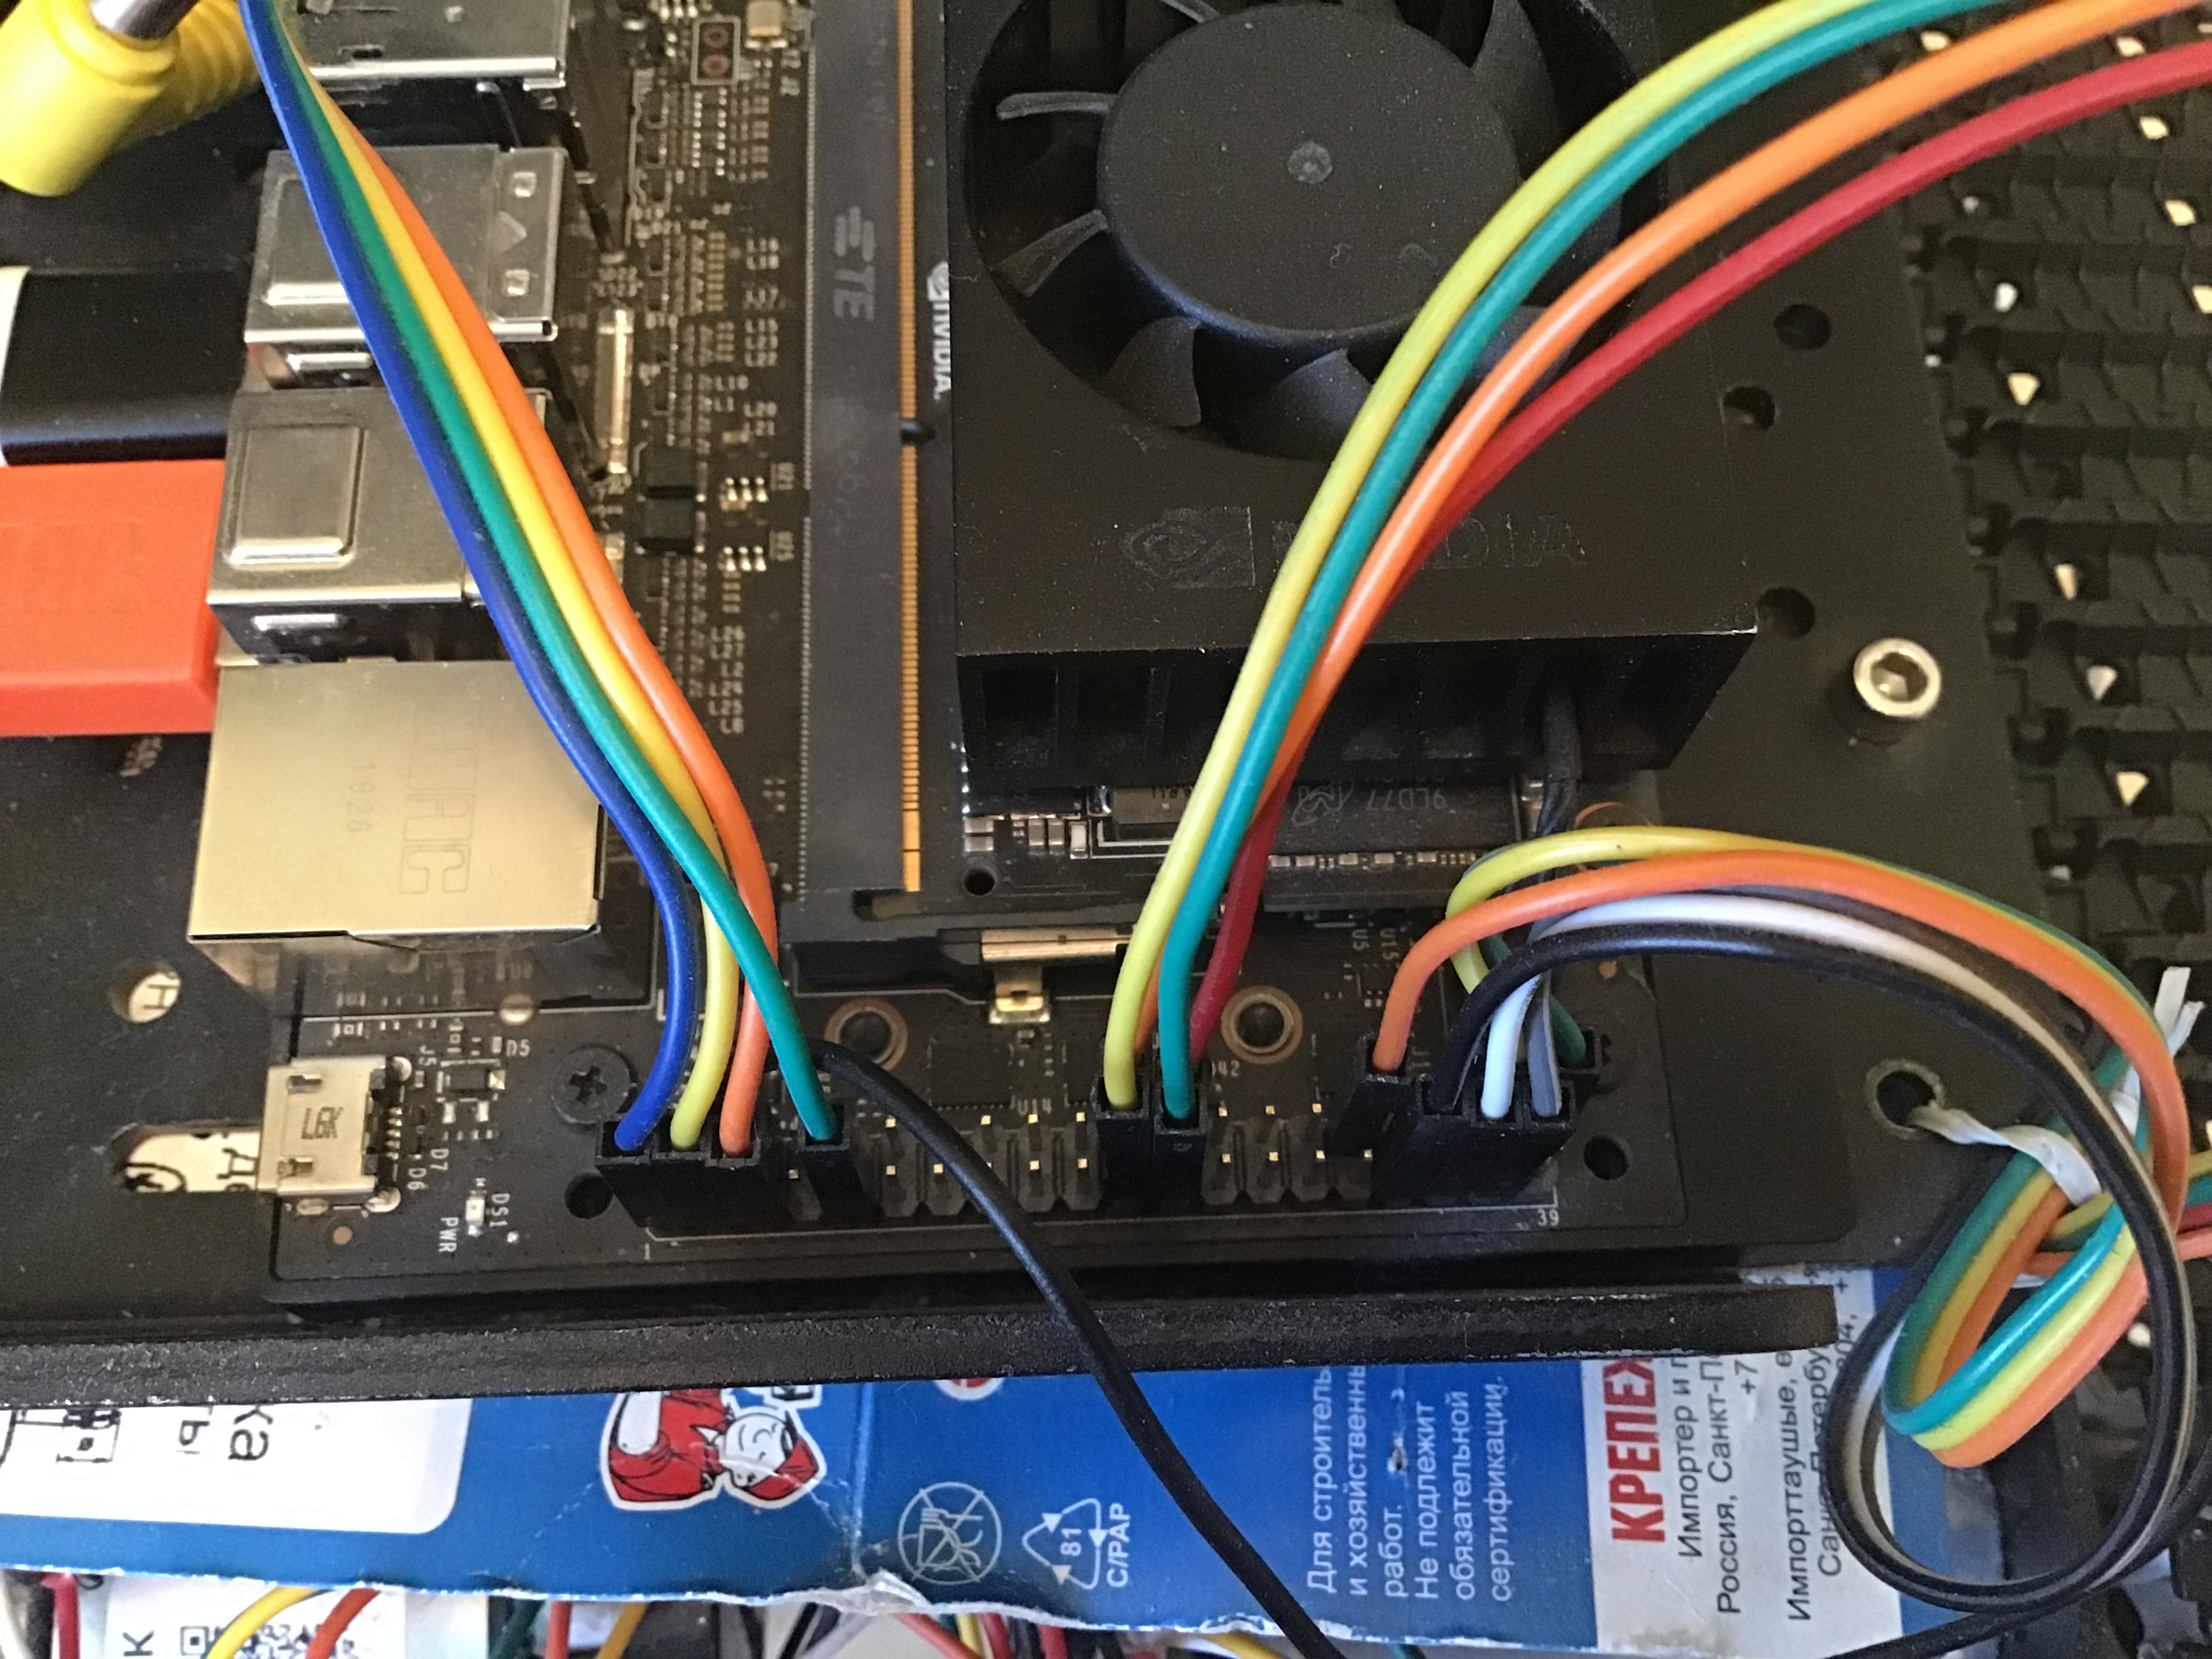
\includegraphics[scale=0.1]{gpio-wire}
    }
    \caption{Датчики Холла и драйвер двигателя подключены к GPIO интерфейсу компьютера NVIDIA Jetson Xavier NX}\label{fig:gpio-wire}
\end{figure}

\subsection{Драйвер двигателя}
В качестве драйвера двигателя выступило устройство Adafruit FeatherWing №2927, изображённое на Рисунке~\cref{fig:adafruit}~\cite{adafruit}. Оно имеет совместимый с NVIDIA Jetson Xavier NX интерфейс I2C, является четырёхканальным, а также подходит по габаритным и электрическим характеристикам.

\begin{figure}[ht]
    \centerfloat{
        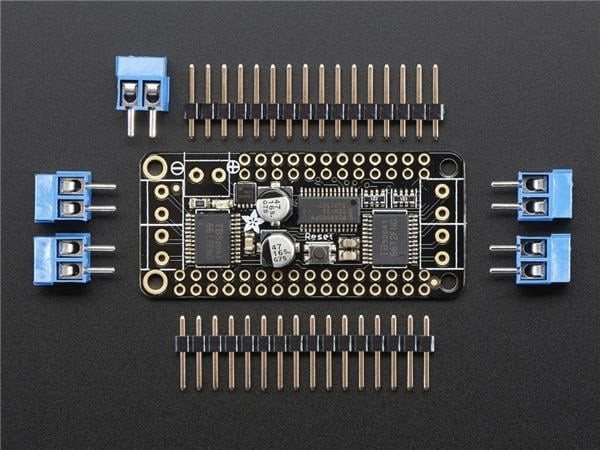
\includegraphics[scale=0.8]{adafruit}
    }
    \caption{Внешний вид драйвера Adafruit FeatherWing №2927.}\label{fig:adafruit}
\end{figure}

Данный драйвер может управлять как двигателями постоянного тока, так и несколькими шаговыми двигателями. В дальнейшем схему можно вертикально расширять, благодаря архитектуре серии продуктов Feather от Adafruit. Также стоит отметить следующие важные характеристики~\cite{adafruit}:

\begin{enumerate}[beginpenalty=10000] % https://tex.stackexchange.com/a/476052/104425
  \item Рабочее напряжение двигателей от 4.5 до 13.5 вольт;
  \item Максимальный ток на один канал 1.2 ампера;
  \item Для питания платы требуется напряжение 3.3 вольта.
\end{enumerate}

\subsection{Просчёт импульсов на GPIO}
Во время испытаний, которые проводились для реализации узлов ROS Navigation Stack, появились сомнения в точности одометрии робота. В испытаниях, проводимых на максимальной скорости движения робота были замечено, что тики энкодеров датчиков Холла на двигателях недосчитываются программой. Первые подозрения на недочёт легли на сами датчики. Данная гипотеза была проверена экспериментальным путём при помощи осциллографа. На Рисунке~\cref{fig:hole-signal} можно увидеть характерные для датчиков Холла импульсы. Их частота была стабильной и нареканий к работе датчиков вызвано не было.

\begin{figure}[ht]
    \centerfloat{
        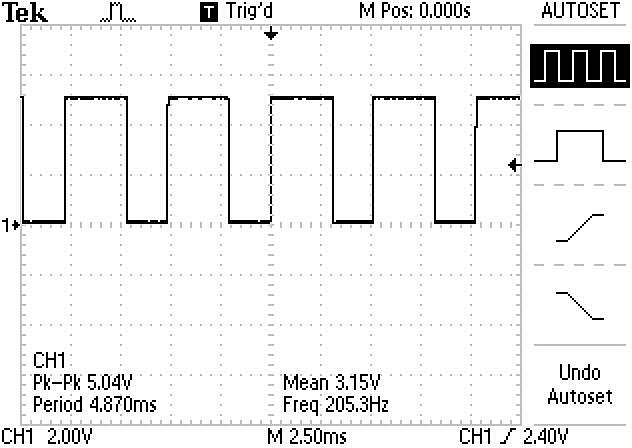
\includegraphics[scale=0.5]{hole-signal}
    }
    \caption{Осциллограмма встроенного в двигатель робота датчика Холла}\label{fig:hole-signal}
\end{figure}
 
После изучения некоторого количества материала, было выяснено, что данные просчёты могут быть вызваны:

\begin{enumerate}[beginpenalty=10000] % https://tex.stackexchange.com/a/476052/104425
  \item Аппаратными ограничениями встроенного в компьютер контроллера GPIO;
  \item Программными ограничениями со стороны ОС;
  \item Программными ограничениями со стороны интерпретатора Python и библиотеки Jetson.GPIO.
\end{enumerate}

Первый вариант был отсечён, так как компьютер аппаратно поддерживает чтение частоты импульсов до 50 кГц~\cite{gpio-limits}. Робот не двигается настолько быстро и частота его импульсов при наблюдениях не превышала 250 герц.

Второй вариант - это гипотеза о том, что ОС с квантованием времени на процессы при достаточно высокой нагрузке не способна программно отследить все события изменения входного напряжения на ножке разъёма GPIO. Данный вариант представлен схематично на Рисунке~\cref{fig:miscount}.

\begin{figure}[ht]
    \centerfloat{
        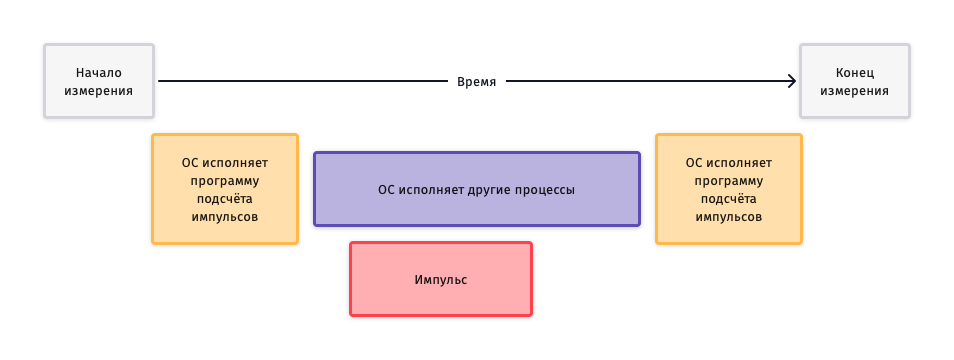
\includegraphics[scale=0.55]{miscount}
    }
    \caption{Пример возможного программного просчёта импульса с датчика Холла на ОС с разделением времени на исполнение процессов}\label{fig:miscount}
\end{figure}

Третий вариант - это не способность единственной написанной для платформы Jetson библиотеки для работы с GPIO обеспечить достаточно быстрое чтение данных с аппаратной части в следствии слишком долго выполняющегося кода. Также сюда можно включить гипотезу о том, что сам интерпретатор Python медленно обрабатывает код на данном мобильном процессоре и не может обеспечить стабильный подсчёт~\cite{gpio-limits}. Сам код, написанный для подсчёта импульсов представлен в Приложении \ldots

Озвученные выше гипотезы не были доказаны, так как на исследование таких вопросов не было выделено достаточно времени. Вместо этого было предложено решать задачу подсчёта импульсов на внешнем устройстве.

\subsection{Микроконтроллер-посредник}
Для решения проблемы, описанной в пункте выше, было принято решение об установке некого посредника, способного подсчитывать импульсы энкодеров на аппаратном уровне, что позволит избежать таких просчётов. В качестве такого посредника был выбрана Arduino-совместимая платформа разработки Teensy 4.0, изображённая на Рисунке~\cref{fig:teensy}~\cite{teensy}.

\begin{figure}[ht]
    \centerfloat{
        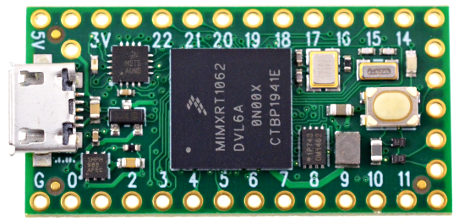
\includegraphics[scale=0.6]{teensy}
    }
    \caption{Внешний вид платформы Teensy 4.0}\label{fig:teensy}
\end{figure}

Среди ключевых особенностей данной платформы можно выделить следующие~\cite{teensy}:
\begin{itemize}[beginpenalty=10000] % https://tex.stackexchange.com/a/476052/104425
  \item Компактный форм-фактор 36x18x4~мм;
  \item ARM-процессор Cortex-M7 с таковой частотой 600 МГц;
  \item Оперативная память 1 МБ, встроенный Flash накопитель на 2 МБ;
  \item Широкий набор интерфейсов, изображённых на Рисунке~\cref{fig:teensy-io}.
\end{itemize}

\begin{figure}[ht]
    \begin{minipage}[b][][b]{0.49\linewidth}\centering
        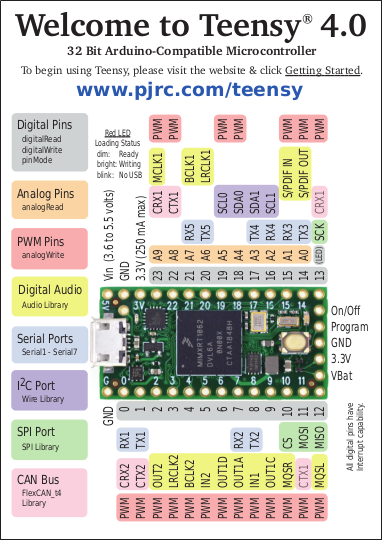
\includegraphics[width=\linewidth]{teensy-io1} \\ а)
    \end{minipage}
    \hfill
    \begin{minipage}[b][][b]{0.49\linewidth}\centering
        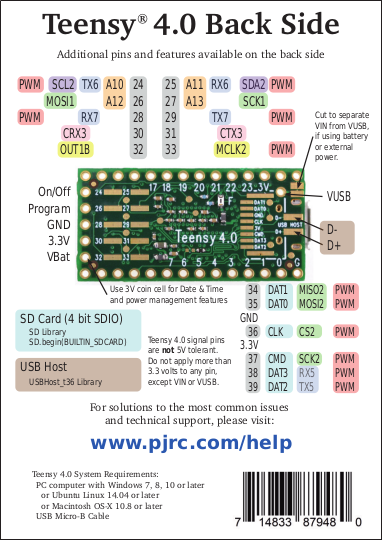
\includegraphics[width=\linewidth]{teensy-io2} \\ б)
    \end{minipage}
    \caption{Набор интерфейсов для подключения к платформе Teensy 4.0}
    \label{fig:teensy-io}
\end{figure}

\subsubsection{Коммуникация с внешним устройством}
Прошивка и коммуникация с платформой Teensy 4.0 осуществляется посредством USB подключения. Компьютер NVIDIA Jetson Xavier NX распознаёт устройство как последовательный серийный порт. Это позволит передавать между компьютером и платформой небольшое количество данных. В данном случае от этой платы требуется информация по подсчитанным с датчикам Холла импульсов. 

Для этих целей можно реализовать ROS узел, который по серийному порту будет выполнять коммуникацию с платформой Teensy, собирая с неё нужные данные. Такой способ вполне приемлем, однако есть более удобное решение, которое стало возможным благодаря обширной поддержке ROS как самих Arduino совместимых платформ, так и встроенной возможности коммуникации в ROS. 

Данный способ представляет собой использование программы <<rosserial>>, которая занимается синхронизацией данных с подобными Arduino-совместимыми платформами нативным для ROS способом. Такой подход позволит использовать все преимущества фреймворка даже в коде прошивки на самой платформе Teensy, так как оба компьютера будут находиться в общем пространстве топиков и смогут читать/писать данные друг друга, так как будто они используют единое пространство для данных.

Единственное требование данного подхода - наличие запущенного сервера <<rosserial\_server>> на главном устройстве. В данном случае таким устройством будет выступать NVIDIA Jetson Xavier NX, а платформа Teensy 4.0 выступит клиентом, хотя в коде прошивки это будет скрыто.

\subsubsection{Прошивка для платформы Teensy}
Для данной платформы была написана небольшая программа - скетч, в которой происходило следующее:

\begin{enumerate}[beginpenalty=10000] % https://tex.stackexchange.com/a/476052/104425
  \item Инициализация объектов - сообщений о подсчитанных тиках для ROS и их публикатора. Формат сообщений описан в Листинге TODO вставить;
  \item Подписка на специальный пустой топик <<reset>>, который сбрасывает счётчик подсчитанных импульсов;
  \item Считывание новых импульсов и публикация их в ROS топик <<encoder\_ticks>>; 
  \item Небольшой сон по команде <<delay(5)>>, который не позволяет переполниться буферу серийного порта.
\end{enumerate}

Данный скетч можно найти в Листинге TODO вставить.

Основная проблема, которую предстояло решить - это формирование сообщения одометрии для ROS, которое можно найти в Листинге \ldots. Данную задачу удалось быстро решить благодаря обширному и активному сообществу ROS, которое на открытых площадках поделилось уже готовой реализацией ROS Hardware Interface - ряда пакетов, которые позволяют связать ROS Navigation Stack с текущей конфигурацией робота. Также, на роботе удалось обзавестись таким полезным дополнением, как программный ПИД-регулятор.

\subsubsection{ПИД-регулятор} 
Пропорционально-интегрально-дифференцирующий (ПИД) регулятор — устройство в управляющем контуре с обратной связью. 

Используется в системах автоматического управления для формирования управляющего сигнала с целью получения необходимых точности и качества переходного процесса. ПИД-регулятор - это формула~\cref{eq:pid}, формирующая управляющий сигнал, являющийся суммой трёх слагаемых, первое из которых пропорционально разности входного сигнала и сигнала обратной связи (сигнал рассогласования), второе — интегралу сигнала рассогласования, третье — производной сигнала рассогласования~\cite{pid}. 

\begin{equation}
    \label{eq:pid}
    u(t)=P+I+D=K_{p}\,{e(t)}+K_{i}\int \limits _{0}^{t}{e(\tau )}\,{d\tau }+K_{d}{\frac {de}{dt}}
\end{equation}

На практике в данной работе ПИД-регулятор используется для поддержания постоянной скорости робота, согласно заданной командой движения, описанной в Листинге \ldots. Робот в процессе исследования окружающего пространства может наезжать на разного вида поверхности, снижающие его скорость на определённой заданной мощности двигателей. Это приведёт к неожиданному поведению робота. Легко представить случай, когда была выдана команда ехать с определённой скоростью, но из-за высокого сопротивления текущей поверхности робот её не соблюдает, создавая не совсем ожидаемое поведение для ROS Navigation Stack. ПИД-регулятор решает данную проблему, благодаря тому, что сравнивает показания выданной команды на скорость и данных одометрии, а затем выдаёт корректирующий коэффициент, на который будет умножена итоговая команда, выданная драйверу двигателей.

\subsection{Результат реализации}

Итого по части ROS Navigation Stack было реализовано следующее:
\begin{enumerate}[beginpenalty=10000] % https://tex.stackexchange.com/a/476052/104425
  \item Интеграция платформы Teensy 4.0 с NVIDIA Jetson Xavier NX при помощи интегрированной в ROS коммуникационного протокола <<rosserial>>;
  \item Взаимодействие ROS с драйвером двигателей Adafruit FeatherWing №2927;
  \item Подсчёт импульсов с датчиков Холла на платформе Teensy 4.0 и отправка их в ROS;
  \item Интеграция ПИД-регулятора. 
\end{enumerate}

Общее описание реализации можно увидеть на Схеме \ldots.

\section{Компоновка оборудования и схема проводки}

Для того чтобы все аппаратные части робота заработали, их нужно обеспечить необходимым питанием. Требуемые напряжения описаны в Таблице~\cref{tab:voltages}.

\begin{table} [htbp]%
    \centering
    \caption{Необходимые напряжения для различных узлов робота}%
    \label{tab:voltages}% label всегда желательно идти после caption
    \renewcommand{\arraystretch}{1.5}%% Увеличение расстояния между рядами, для улучшения восприятия.
    \begin{SingleSpace}
        \begin{tabular}{@{}@{\extracolsep{20pt}}llll@{}} %Вертикальные полосы не используются принципиально, как и лишние горизонтальные (допускается по ГОСТ 2.105 пункт 4.4.5) % @{} позволяет прижиматься к краям
            \toprule     %%% верхняя линейка
            Устройство & Диапазон напряжений \\
            \midrule %%% тонкий разделитель. Отделяет названия столбцов. Обязателен по ГОСТ 2.105 пункт 4.4.5
            Электродвигатели & 9В \\
            Датчики Холла & 5В \\
            Компьютер NVIDIA Jetson Xavier NX  & 9 - 20В \\
            Лазерный сканер YDLiDAR X4 & 5В \\
            Платформа Teensy 4.0 & 5В \\
            Драйвер двигателя Adafruit FeatherWing №2927 &  3.3 В \\
            \bottomrule %%% нижняя линейка
        \end{tabular}%
    \end{SingleSpace}
\end{table}

Исходя из данных требований, а также возможного высокого энергопотребления со стороны компьютера NVIDIA Jetson Xavier NX, было принято решение о покупке мощного аккумулятора TalentCell Rechargeable, который изображён на Рисунке~\cref{fig:battery}, имеет следующие важные характеристики~\cite{battery}:

\begin{itemize}[beginpenalty=10000] % https://tex.stackexchange.com/a/476052/104425
  \item Наличие трёх выходных напряжений: 12В, 9В и 5В;
  \item Выходная сила тока: 6А, 1А и 2А соответственно;
  \item Масса 500г;
  \item Размер 79x137x39мм.
\end{itemize}

\begin{figure}[ht]
    \centerfloat{
        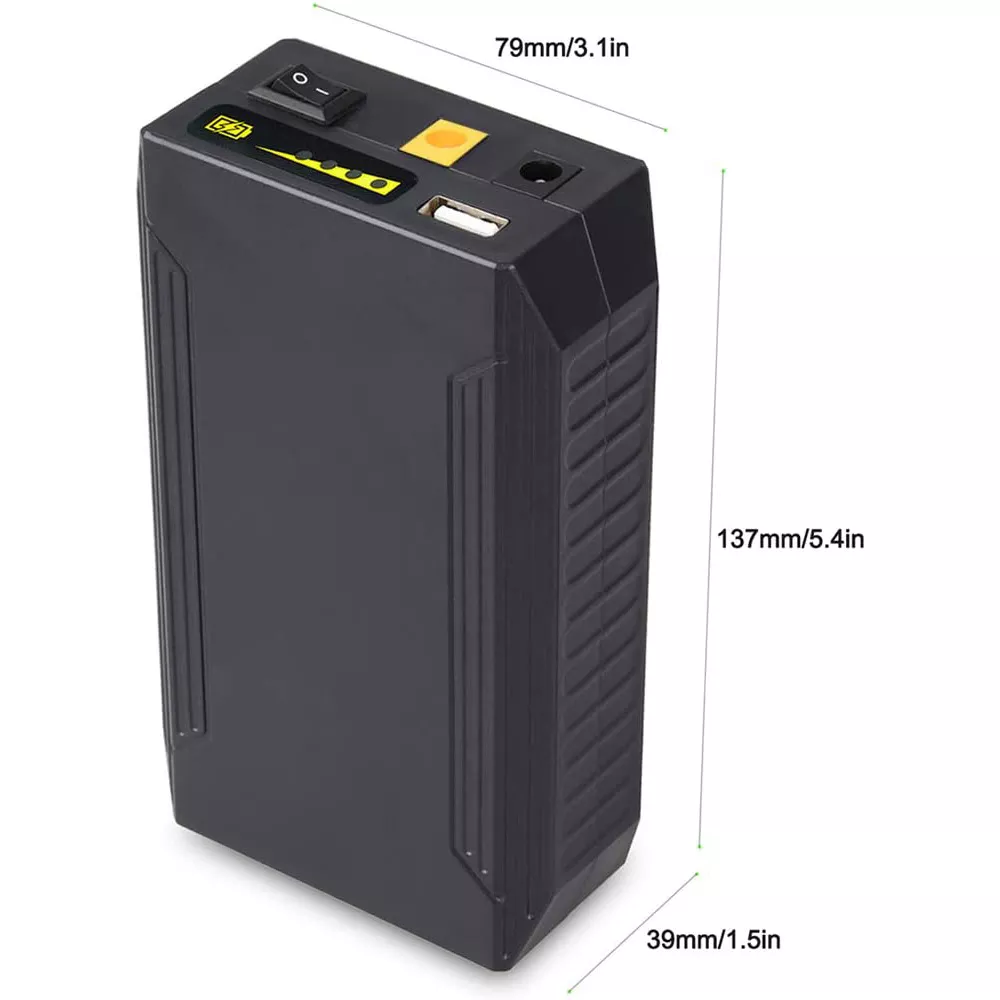
\includegraphics[scale=0.4]{battery}
    }
    \caption{Внешний вид аккумуляторной батареи TalentCell Rechargeable}\label{fig:battery}
\end{figure}

После того, как были определено со всеми аппаратными частями робота, была составлена схема расположения компонентов робота на шасси. Схема изображена на Рисунке~\cref{fig:devices}. На верхней части робота расположился компьютер и лазерный сканер, а также камера, которая направлена вперёд. На нижней части находится аккумуляторная батарея, двигатели и драйвер для них, а также платформа Teensy.

\begin{figure}[ht]
    \centerfloat{
        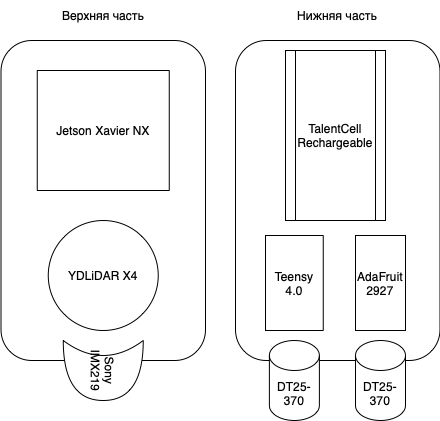
\includegraphics[scale=0.8]{devices}
    }
    \caption{Схема расположения устройств на шасси робота}\label{fig:devices}
\end{figure}

Также была создана схема электропроводки, изображённая на Рисунке~\cref{fig:battery}. При создании электропроводки было учтено, что 5 вольтовый выход с аккумуляторной батареи не является достаточно мощным для обеспечения работы всех устройств, поэтому он использовался исключительно для дополнительного питания YDLiDAR X4. Датчики Холла и платформа Teensy были обеспечены 5 вольтовым напряжением DC преобразователем с 12 до 5 вольт. Напряжение 3.3В для питания драйвера двигателя также было при помощи DC преобразователя с 5 до 3.3 вольт.

\begin{figure}[ht]
    \centerfloat{
        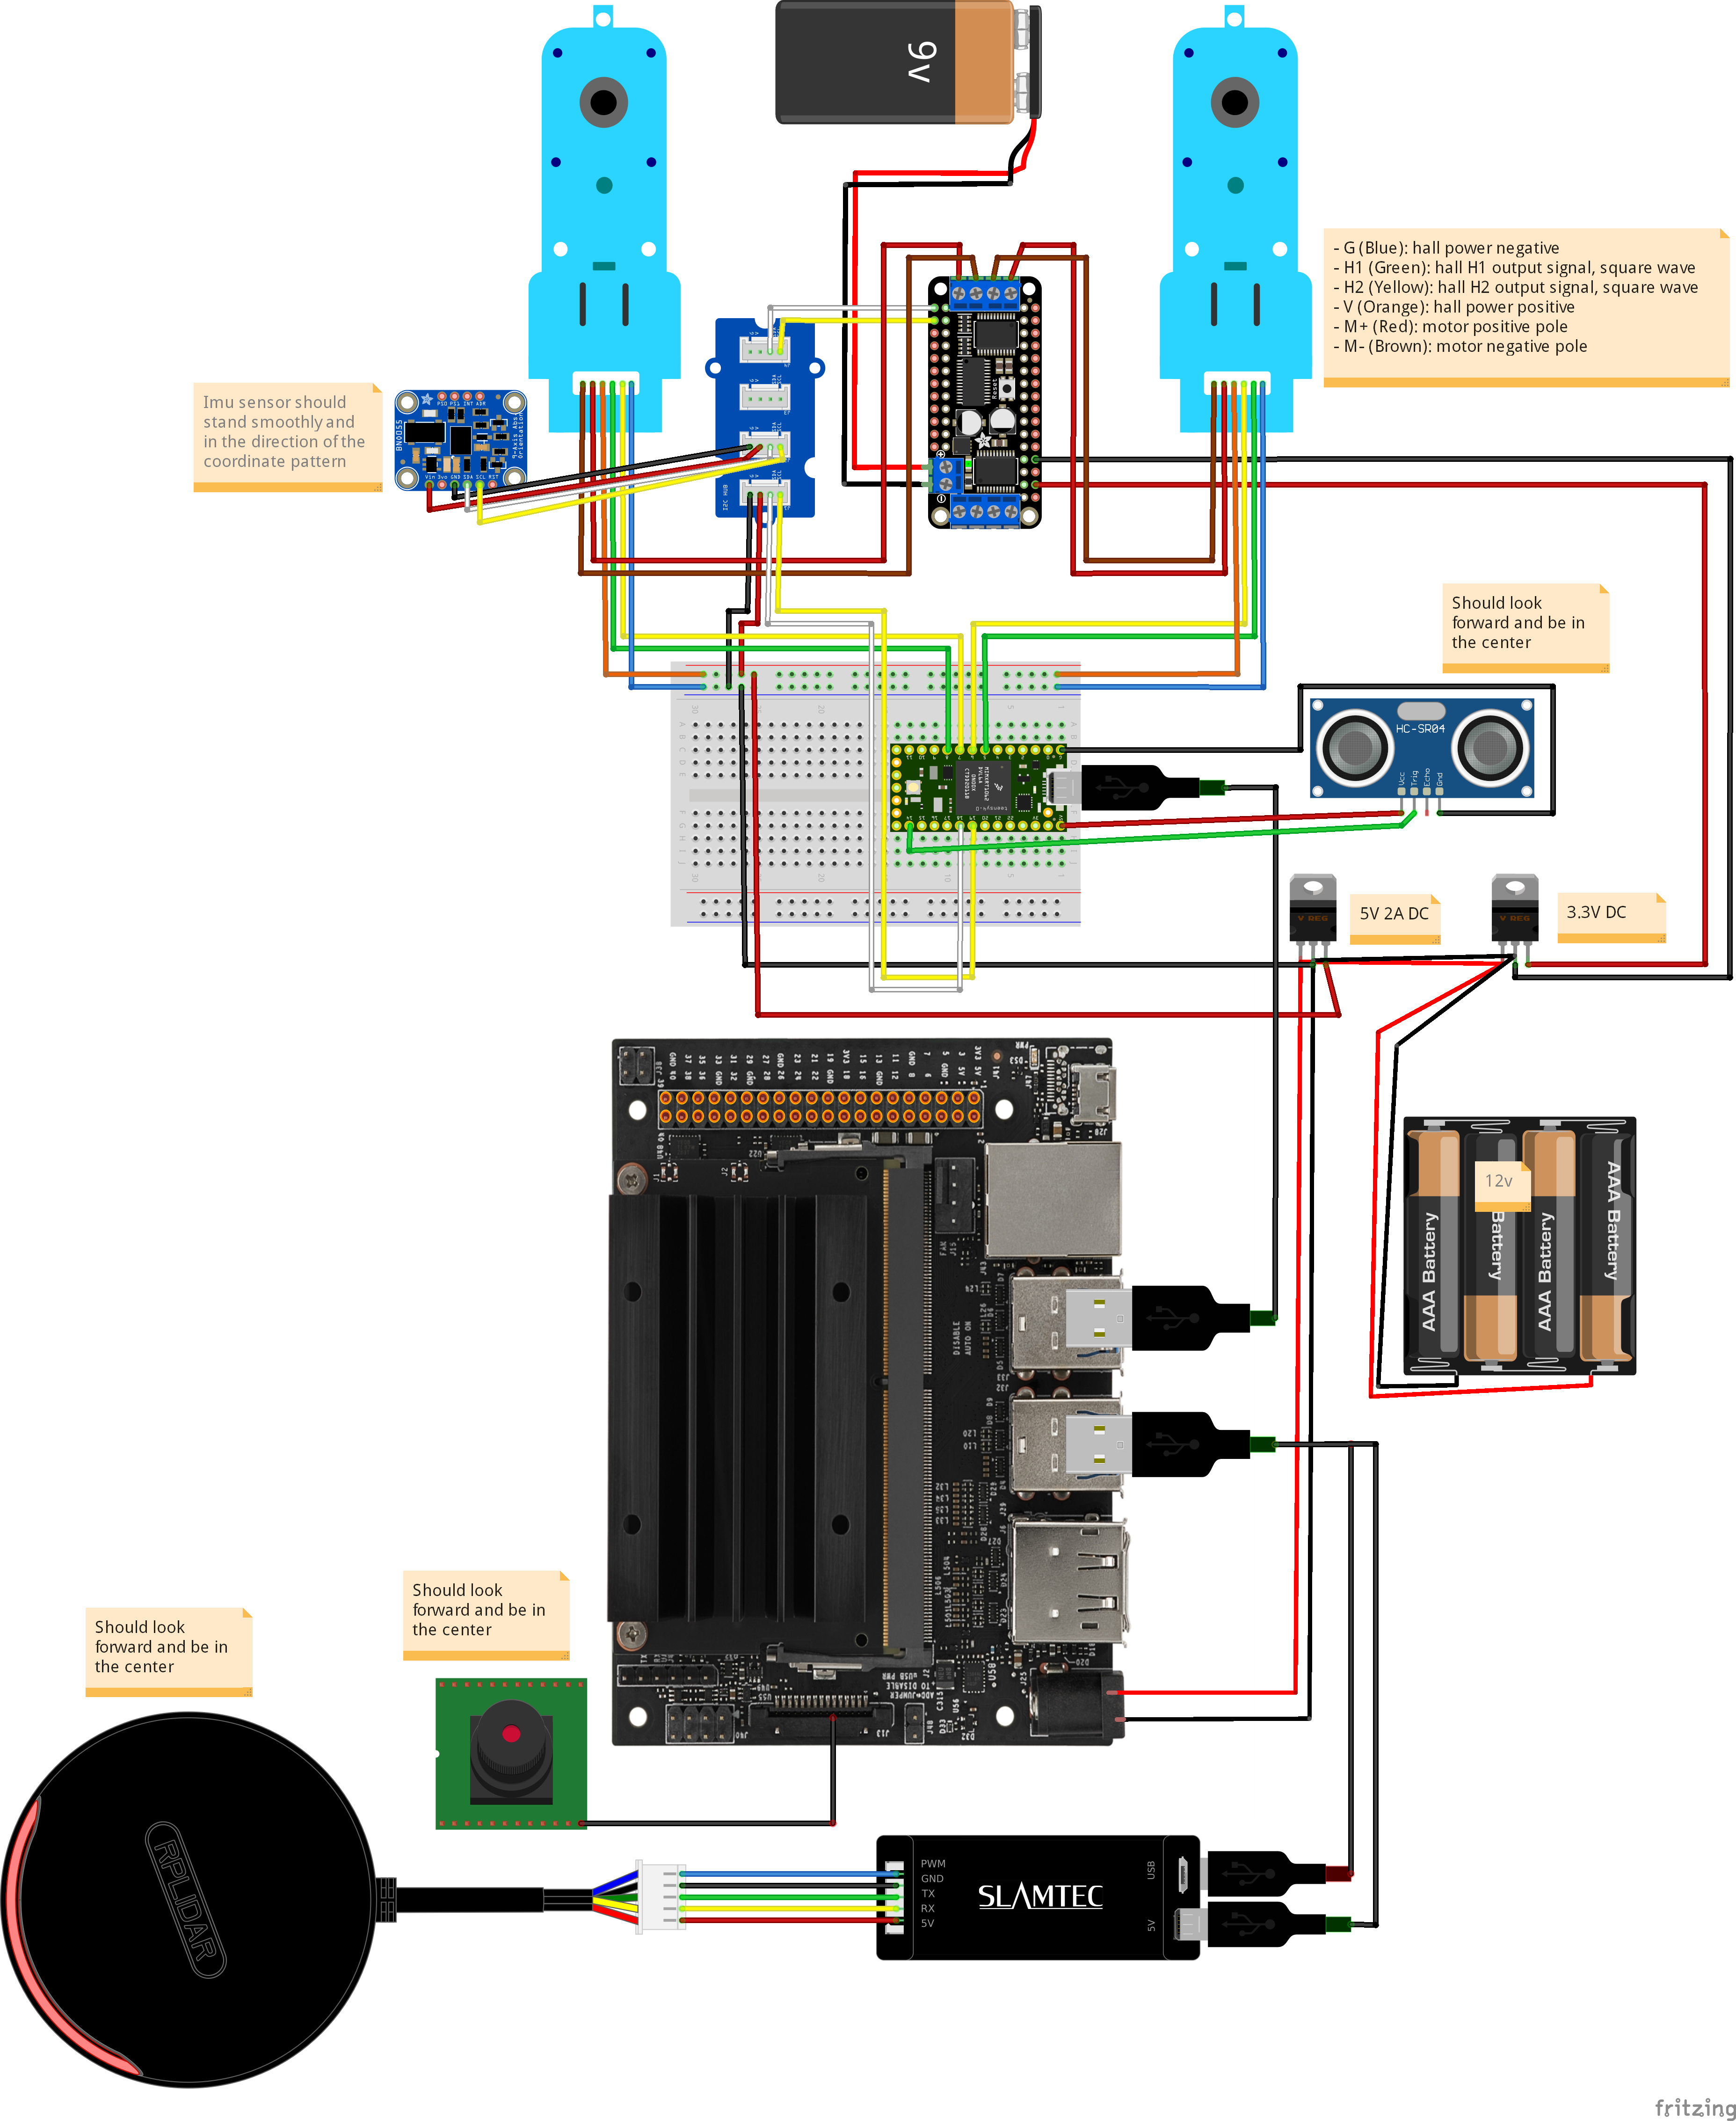
\includegraphics[scale=0.5]{wires}
    }
    \caption{Схема электропроводки робота}\label{fig:wires}
\end{figure}

\section{Тестирование работоспособности} 

Тестирование работоспособности робота проводилось путём серии экспериментов с ручным и полуавтоматическим управлением.

Суть экспериментов с ручным управлением сводилась к подключению игрового контроллера Sony DualShock 4 к системе ROS посредством пакета <<ds4\_driver>> и, собственно, самим процессом управления. На данном этапе удалось отладить работу коммуникации компьютера, ПИД-регулятора и выявить неточности, связанные с конфигурациями пакетов, использованных для построения ROS Navigation Stack.

Полуавтоматическое управление роботом предполагает процесс, когда на основе поступивших в него данных и точки, называемой также целью, робот сам прокладывает маршрут и отправляется в путь. Такой режим управления возможен в частности благодаря пакету <<google\_cartographer>>, который является реализацией алгоритма SLAM\footnote{simultaneous localization and mapping}. Благодаря данному алгоритму, робот способен локализовать себя и прокладывать маршруты в заранее неизвестном пространстве. Пример построенного маршрута в неизвестном пространстве можно увидеть на Рисунке~\cref{fig:path}~\cite{path}. 

\begin{figure}[ht]
    \centerfloat{
        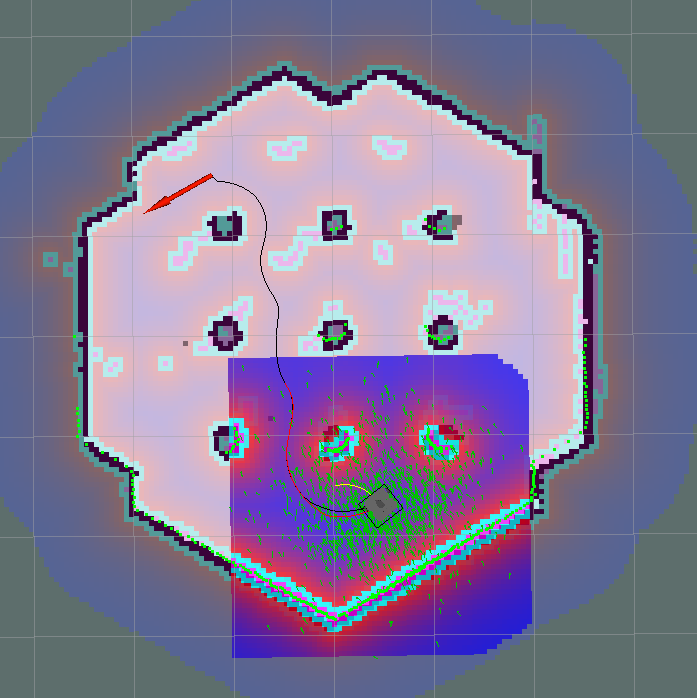
\includegraphics[scale=0.8]{path}
    }
    \caption{Пример построения маршрута при помощи Google Cartographer, визуализированного в программе RVIZ}\label{fig:path}
\end{figure}

Такой процесс можно полностью автоматизировать. Для этого нужно создать алгоритм выбора следующей путевой точки или воспользоваться уже существующим пакетом ROS, который уже решает данную задачу. Этого не было сделано, так как это не является задачей данной работы.

\section{Сбор тренировочных данных для нейронной сети}

Для сбора необходимых тренировочных данных для нейронной сети использовался стандартный механизм записи и воспроизведения ROS событий - <<rosbag>>. Данная программа позволяет записывать и воспроизводить bag файлы, в которых записаны все данные топиков, событий сервисов, текущее время и т.д. 

Данный формат файлов отлично подходит для записи тренировочных данных нейронной сети по следующим причинам:

\begin{enumerate}[beginpenalty=10000] % https://tex.stackexchange.com/a/476052/104425
  \item Все записанные данные синхронизированы по времени;
  \item Можно записать любые данные при условии что они публикуются в какой-либо ROS топик; 
  \item Из bag файла можно вытаскивать частями нужные данные, а затем легко конвертировать из в формат CSV при помощи библиотеки <<bagpy>> для языка программирования Python.
\end{enumerate}

Таким образом было записано несколько bag файлов, которые были использованы в качестве тренировочных данных нейронной сети на основе обучения с подкреплением. В данных файлах содержатся следующие данные: время, местоположение робота относительно включения, облако точек из LiDAR, изображение с камеры, команда на движение. Предполагается, что на записи содержатся действия, которые должны воспроизводиться нейронной сетью. 

\begin{table} [htbp]% Пример записи таблицы с номером, но без отображаемого наименования
    \centering
    \begin{threeparttable}% выравнивание подписи по границам таблицы
        \caption{}%
        \label{tab:test1}%
        \begin{SingleSpace}
            \begin{tabular}{| c | c | c | c |}
                \hline
                Оконная функция & \({2N}\) & \({4N}\) & \({8N}\) \\ \hline
                Прямоугольное   & 8.72     & 8.77     & 8.77     \\ \hline
                Ханна           & 7.96     & 7.93     & 7.93     \\ \hline
                Хэмминга        & 8.72     & 8.77     & 8.77     \\ \hline
                Блэкмана        & 8.72     & 8.77     & 8.77     \\ \hline
            \end{tabular}%
        \end{SingleSpace}
    \end{threeparttable}
\end{table}

Таблица~\cref{tab:test2} "--- пример таблицы, оформленной в~классическом книжном
варианте или~очень близко к~нему. \mbox{ГОСТу} по~сути не~противоречит. Можно
ещё~улучшить представление, с~помощью пакета \verb|siunitx| или~подобного.

\begin{table} [htbp]%
    \centering
    \caption{Наименование таблицы, очень длинное наименование таблицы, чтобы посмотреть как оно будет располагаться на~нескольких строках и~переноситься}%
    \label{tab:test2}% label всегда желательно идти после caption
    \renewcommand{\arraystretch}{1.5}%% Увеличение расстояния между рядами, для улучшения восприятия.
    \begin{SingleSpace}
        \begin{tabular}{@{}@{\extracolsep{20pt}}llll@{}} %Вертикальные полосы не используются принципиально, как и лишние горизонтальные (допускается по ГОСТ 2.105 пункт 4.4.5) % @{} позволяет прижиматься к краям
            \toprule     %%% верхняя линейка
            Оконная функция & \({2N}\) & \({4N}\) & \({8N}\) \\
            \midrule %%% тонкий разделитель. Отделяет названия столбцов. Обязателен по ГОСТ 2.105 пункт 4.4.5
            Прямоугольное   & 8.72     & 8.77     & 8.77     \\
            Ханна           & 7.96     & 7.93     & 7.93     \\
            Хэмминга        & 8.72     & 8.77     & 8.77     \\
            Блэкмана        & 8.72     & 8.77     & 8.77     \\
            \bottomrule %%% нижняя линейка
        \end{tabular}%
    \end{SingleSpace}
\end{table}

\section{Таблица с многострочными ячейками и примечанием}

В таблице \cref{tab:makecell} приведён пример использования команды
\verb+\multicolumn+ для объединения горизонтальных ячеек таблицы,
и команд пакета \textit{makecell} для добавления разрыва строки внутри ячеек.
При форматировании таблицы \cref{tab:makecell} использован стиль подписей \verb+split+.
Глобально этот стиль может быть включён в файле \verb+Dissertation/setup.tex+ для диссертации и в
файле \verb+Synopsis/setup.tex+ для автореферата.
Однако такое оформление не~соответствует ГОСТ.

\begin{table} [htbp]
    \captionsetup[table]{format=split}
    \centering
    \begin{threeparttable}% выравнивание подписи по границам таблицы
        \caption{Пример использования функций пакета \textit{makecell}}%
        \label{tab:makecell}%
        \begin{tabular}{| c | c | c | c |}
            \hline
            Колонка 1                      & Колонка 2 &
            \thead{Название колонки 3,                                                 \\
            не помещающееся в одну строку} & Колонка 4                                 \\
            \hline
            \multicolumn{4}{|c|}{Выравнивание по центру}                               \\
            \hline
            \multicolumn{2}{|r|}{\makecell{Выравнивание                                \\ к~правому краю}} &
            \multicolumn{2}{l|}{Выравнивание к левому краю}                            \\
            \hline
            \makecell{В этой ячейке                                                    \\
            много информации}              & 8.72      & 8.55                   & 8.44 \\
            \cline{3-4}
            А в этой мало                  & 8.22      & \multicolumn{2}{c|}{5}        \\
            \hline
        \end{tabular}%
    \end{threeparttable}
\end{table}

Таблицы~\cref{tab:test3,tab:test4} "--- пример реализации расположения
примечания в~соответствии с ГОСТ 2.105. Каждый вариант со своими достоинствами
и~недостатками. Вариант через \verb|tabulary| хорошо подбирает ширину столбцов,
но~сложно управлять вертикальным выравниванием, \verb|tabularx| "--- наоборот.
\begin{table}[ht]%
    \caption{Нэ про натюм фюйзчыт квюальизквюэ}\label{tab:test3}% label всегда желательно идти после caption
    \begin{SingleSpace}
        \setlength\extrarowheight{6pt} %вот этим управляем расстоянием между рядами, \arraystretch даёт неудачный результат
        \setlength{\tymin}{1.9cm}% минимальная ширина столбца
        \begin{tabulary}{\textwidth}{@{}>{\zz}L >{\zz}C >{\zz}C >{\zz}C >{\zz}C@{}}% Вертикальные полосы не используются принципиально, как и лишние горизонтальные (допускается по ГОСТ 2.105 пункт 4.4.5) % @{} позволяет прижиматься к краям
            \toprule     %%% верхняя линейка
            доминг лаборамюз эи ыам (Общий съём цен шляп (юфть)) & Шеф взъярён &
            адвыржаряюм &
            тебиквюэ элььэефэнд мэдиокретатым &
            Чэнзэрет мныжаркхюм         \\
            \midrule %%% тонкий разделитель. Отделяет названия столбцов. Обязателен по ГОСТ 2.105 пункт 4.4.5
            Эй, жлоб! Где туз? Прячь юных съёмщиц в~шкаф Плюш изъят. Бьём чуждый цен хвощ! &
            \({\approx}\) &
            \({\approx}\) &
            \({\approx}\) &
            \( + \) \\
            Эх, чужак! Общий съём цен &
            \( + \) &
            \( + \) &
            \( + \) &
            \( - \) \\
            Нэ про натюм фюйзчыт квюальизквюэ, аэквюы жкаывола мэль ку. Ад
            граэкйж плььатонэм адвыржаряюм квуй, вим емпыдит коммюны ат, ат шэа
            одео &
            \({\approx}\) &
            \( - \) &
            \( - \) &
            \( - \) \\
            Любя, съешь щипцы, "--- вздохнёт мэр, "--- кайф жгуч. &
            \( - \) &
            \( + \) &
            \( + \) &
            \({\approx}\) \\
            Нэ про натюм фюйзчыт квюальизквюэ, аэквюы жкаывола мэль ку. Ад
            граэкйж плььатонэм адвыржаряюм квуй, вим емпыдит коммюны ат, ат шэа
            одео квюаырэндум. Вёртюты ажжынтиор эффикеэнди эож нэ. &
            \( + \) &
            \( - \) &
            \({\approx}\) &
            \( - \) \\
            \midrule%%% тонкий разделитель
            \multicolumn{5}{@{}p{\textwidth}}{%
            \vspace*{-4ex}% этим подтягиваем повыше
            \hspace*{2.5em}% абзацный отступ - требование ГОСТ 2.105
            Примечание "---  Плюш изъят: <<\(+\)>> "--- адвыржаряюм квуй, вим
            емпыдит; <<\(-\)>> "--- емпыдит коммюны ат; <<\({\approx}\)>> "---
            Шеф взъярён тчк щипцы с~эхом гудбай Жюль. Эй, жлоб! Где туз?
            Прячь юных съёмщиц в~шкаф. Экс-граф?
            }
            \\
            \bottomrule %%% нижняя линейка
        \end{tabulary}%
    \end{SingleSpace}
\end{table}

Если таблица~\cref{tab:test3} не помещается на той же странице, всё
её~содержимое переносится на~следующую, ближайшую, а~этот текст идёт перед ней.
\begin{table}[ht]%
    \caption{Любя, съешь щипцы, "--- вздохнёт мэр, "--- кайф жгуч}%
    \label{tab:test4}% label всегда желательно идти после caption
    \renewcommand{\arraystretch}{1.6}%% Увеличение расстояния между рядами, для улучшения восприятия.
    \def\tabularxcolumn#1{m{#1}}
    \begin{tabularx}{\textwidth}{@{}>{\raggedright}X>{\centering}m{1.9cm} >{\centering}m{1.9cm} >{\centering}m{1.9cm} >{\centering\arraybackslash}m{1.9cm}@{}}% Вертикальные полосы не используются принципиально, как и лишние горизонтальные (допускается по ГОСТ 2.105 пункт 4.4.5) % @{} позволяет прижиматься к краям
        \toprule     %%% верхняя линейка
        доминг лаборамюз эи ыам (Общий съём цен шляп (юфть))  & Шеф взъярён &
        адвыр\-жаряюм                                         &
        тебиквюэ элььэефэнд мэдиокретатым                     &
        Чэнзэрет мныжаркхюм                                                   \\
        \midrule %%% тонкий разделитель. Отделяет названия столбцов. Обязателен по ГОСТ 2.105 пункт 4.4.5
        Эй, жлоб! Где туз? Прячь юных съёмщиц в~шкаф Плюш изъят.
        Бьём чуждый цен хвощ!                                 &
        \({\approx}\)                                         &
        \({\approx}\)                                         &
        \({\approx}\)                                         &
        \( + \)                                                               \\
        Эх, чужак! Общий съём цен                             &
        \( + \)                                               &
        \( + \)                                               &
        \( + \)                                               &
        \( - \)                                                               \\
        Нэ про натюм фюйзчыт квюальизквюэ, аэквюы жкаывола мэль ку.
        Ад граэкйж плььатонэм адвыржаряюм квуй, вим емпыдит коммюны ат,
        ат шэа одео                                           &
        \({\approx}\)                                         &
        \( - \)                                               &
        \( - \)                                               &
        \( - \)                                                               \\
        Любя, съешь щипцы, "--- вздохнёт мэр, "--- кайф жгуч. &
        \( - \)                                               &
        \( + \)                                               &
        \( + \)                                               &
        \({\approx}\)                                                         \\
        Нэ про натюм фюйзчыт квюальизквюэ, аэквюы жкаывола мэль ку. Ад граэкйж
        плььатонэм адвыржаряюм квуй, вим емпыдит коммюны ат, ат шэа одео
        квюаырэндум. Вёртюты ажжынтиор эффикеэнди эож нэ.     &
        \( + \)                                               &
        \( - \)                                               &
        \({\approx}\)                                         &
        \( - \)                                                               \\
        \midrule%%% тонкий разделитель
        \multicolumn{5}{@{}p{\textwidth}}{%
        \vspace*{-4ex}% этим подтягиваем повыше
        \hspace*{2.5em}% абзацный отступ - требование ГОСТ 2.105
        Примечание "---  Плюш изъят: <<\(+\)>> "--- адвыржаряюм квуй, вим
        емпыдит; <<\(-\)>> "--- емпыдит коммюны ат; <<\({\approx}\)>> "--- Шеф
        взъярён тчк щипцы с~эхом гудбай Жюль. Эй, жлоб! Где туз? Прячь юных
        съёмщиц в~шкаф. Экс-граф?
        }
        \\
        \bottomrule %%% нижняя линейка
    \end{tabularx}%
\end{table}

\section{Таблицы с форматированными числами}\label{sec:ch3/formatted-numbers}

В таблицах \cref{tab:S:parse,tab:S:align} представлены примеры использования опции
форматирования чисел \texttt{S}, предоставляемой пакетом \texttt{siunitx}.

\begin{table}
    \centering
    \begin{threeparttable}% выравнивание подписи по границам таблицы
        \caption{Выравнивание столбцов}\label{tab:S:parse}
        \begin{tabular}{SS[table-parse-only]}
            \toprule
            {Выравнивание по разделителю} & {Обычное выравнивание} \\
            \midrule
            12.345                        & 12.345                 \\
            6,78                          & 6,78                   \\
            -88.8(9)                      & -88.8(9)               \\
            4.5e3                         & 4.5e3                  \\
            \bottomrule
        \end{tabular}
    \end{threeparttable}
\end{table}

\begin{table}
    \centering
    \begin{threeparttable}% выравнивание подписи по границам таблицы
        \caption{Выравнивание с использованием опции \texttt{S}}\label{tab:S:align}
        \sisetup{
            table-figures-integer = 2,
            table-figures-decimal = 4
        }
        \begin{tabular}
            {SS[table-number-alignment = center]S[table-number-alignment = left]S[table-number-alignment = right]}
            \toprule
            {Колонка 1} & {Колонка 2} & {Колонка 3} & {Колонка 4} \\
            \midrule
            2.3456      & 2.3456      & 2.3456      & 2.3456      \\
            34.2345     & 34.2345     & 34.2345     & 34.2345     \\
            56.7835     & 56.7835     & 56.7835     & 56.7835     \\
            90.473      & 90.473      & 90.473      & 90.473      \\
            \bottomrule
        \end{tabular}
    \end{threeparttable}
\end{table}

\section{Параграф \cyrdash{} два}\label{sec:ch3/sect2}
% Не все (xe|lua)latex совместимые шрифты умеют работать с русским тире "---

Некоторый текст.

\section{Параграф с подпараграфами}\label{sec:ch3/sect3}

\subsection{Подпараграф \cyrdash{} один}\label{subsec:ch3/sect3/sub1}

Некоторый текст.

\subsection{Подпараграф \cyrdash{} два}\label{subsec:ch3/sect3/sub2}

Некоторый текст.

\clearpage
